% GENERATED BY sshrc_figures.py - edit that file, not this one.
% The document that inputs this file supplies the float, the caption and the label.
% Stream B. Committees, left to right within each year: Economics, Business (14A, 14B, 14C), Multidisciplinary humanities, Multidisciplinary social sciences (23, 23A, 23B).
\definecolor{sshrcA}{HTML}{2A78D6}
\definecolor{sshrcB}{HTML}{EB6834}
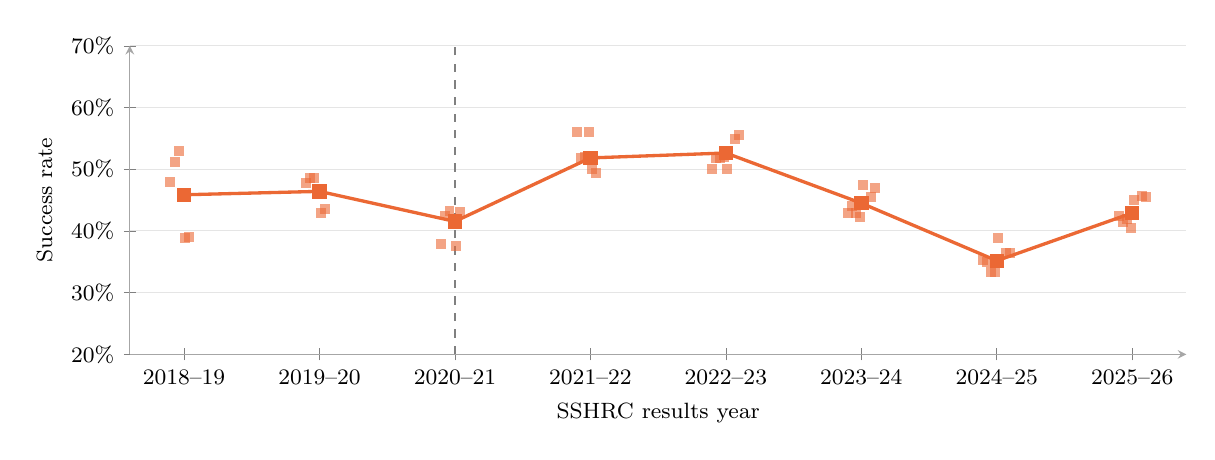
\begin{tikzpicture}
\begin{axis}[
  width=15cm, height=5.5cm,
  xmin=2017.6, xmax=2025.4, ymin=20, ymax=70,
  xtick={2018,2019,2020,2021,2022,2023,2024,2025}, xticklabels={2018--19,2019--20,2020--21,2021--22,2022--23,2023--24,2024--25,2025--26},
  axis x line=bottom, axis y line=left, axis line style={gray!70},
  ymajorgrids, grid style={gray!20},
  tick label style={font=\footnotesize}, label style={font=\footnotesize},
  xlabel={SSHRC results year}, ylabel={Success rate}, ylabel style={align=center},
  clip=false,
  ytick distance=10, yticklabel={\pgfmathprintnumber{\tick}\%},
]
\draw[gray, dashed, line width=0.7pt] (axis cs:2020,20) -- (axis cs:2020,70);
\addplot[only marks, mark=square*, mark size=1.8pt, color=sshrcB,
  mark options={fill opacity=0.6, draw opacity=0}]
  coordinates {(2017.93,51.11) (2017.96,52.94) (2017.90,48.00) (2018.01,38.89) (2018.04,38.98) (2018.93,48.57) (2018.96,48.57) (2018.90,47.83) (2019.01,42.86) (2019.04,43.48) (2019.90,37.93) (2019.93,42.50) (2019.96,43.18) (2020.01,37.50) (2020.04,43.10) (2020.90,56.00) (2020.93,51.85) (2020.96,52.00) (2020.99,56.00) (2021.01,50.00) (2021.04,49.32) (2021.90,50.00) (2021.93,51.85) (2021.96,51.85) (2021.99,52.00) (2022.01,50.00) (2022.07,54.84) (2022.10,55.56) (2022.90,42.86) (2022.93,44.00) (2022.96,42.86) (2022.99,42.31) (2023.01,47.37) (2023.07,45.45) (2023.10,46.88) (2023.90,35.29) (2023.93,35.00) (2023.96,33.33) (2023.99,33.33) (2024.01,38.89) (2024.07,36.36) (2024.10,36.36) (2024.90,42.42) (2024.93,41.46) (2024.96,41.86) (2024.99,40.48) (2025.01,45.00) (2025.07,45.71) (2025.10,45.45)};
\addplot[color=sshrcB, line width=1.2pt, mark=square*, mark size=2pt] coordinates {(2018.00,45.86) (2019.00,46.41) (2020.00,41.54) (2021.00,51.83) (2022.00,52.63) (2023.00,44.50) (2024.00,35.17) (2025.00,42.91)};
\end{axis}
\end{tikzpicture}
